\documentclass[journal,12pt,twocolumn]{IEEEtran}
%
\usepackage{setspace}
\usepackage{multicol}
\usepackage{gensymb}
\usepackage{enumerate}
\usepackage{xcolor}
\usepackage{caption}
%\usepackage{subcaption}
%\doublespacing
\singlespacing
%\usepackage{epstopdf}
%\usepackage{graphicx}
%\usepackage{amssymb}
%\usepackage{relsize}
\usepackage[cmex10]{amsmath}
\usepackage{mathtools}
%\usepackage{amsthm}
%\interdisplaylinepenalty=2500
%\savesymbol{iint}
%\usepackage{txfonts}
%\restoresymbol{TXF}{iint}
%\usepackage{wasysym}
\usepackage{amsthm}
\usepackage{mathrsfs}
\usepackage{txfonts}
\usepackage{stfloats}
\usepackage{cite}
\usepackage{cases}
\usepackage{subfig}
%\usepackage{xtab}
\usepackage{longtable}
\usepackage{multirow}
%\usepackage{algorithm}
%\usepackage{algpseudocode}
%\usepackage{enumitem}
\usepackage{mathtools}
\usepackage{iithtlc}
%\usepackage[framemethod=tikz]{mdframed}
\usepackage{listings}
\usepackage{amsmath}
\usepackage{polynomial}

%\usepackage{stmaryrd}


%\usepackage{wasysym}
%\newcounter{MYtempeqncnt}
\DeclareMathOperator*{\Res}{Res}
%\renewcommand{\baselinestretch}{2}
\renewcommand\thesection{\arabic{section}}
\renewcommand\thesubsection{\thesection.\arabic{subsection}}
\renewcommand\thesubsubsection{\thesubsection.\arabic{subsubsection}}

\renewcommand\thesectiondis{\arabic{section}}
\renewcommand\thesubsectiondis{\thesectiondis.\arabic{subsection}}
\renewcommand\thesubsubsectiondis{\thesubsectiondis.\arabic{subsubsection}}

% correct bad hyphenation here
\hyphenation{op-tical net-works semi-conduc-tor}

\lstset{
language=Python,
frame=single, 
breaklines=true
}

%\lstset{
	%%basicstyle=\small\ttfamily\bfseries,
	%%numberstyle=\small\ttfamily,
	%language=python,
	%backgroundcolor=\color{white},
	%%frame=single,
	%%keywordstyle=\bfseries,
	%%breaklines=true,
	%%showstringspaces=false,
	%%xleftmargin=-10mm,
	%%aboveskip=-1mm,
	%%belowskip=0mm
%}

%\surroundwithmdframed[width=\columnwidth]{lstlisting}


\begin{document}
%

\theoremstyle{definition}
\newtheorem{theorem}{Theorem}[section]
%\newtheorem{problem}{Problem}[section]
\newtheorem{problem}{Problem}
\newtheorem{proposition}{Proposition}
%\newtheorem{proposition}{Proposition}[section]
\newtheorem{lemma}{Lemma}[section]
\newtheorem{corollary}[theorem]{Corollary}
\newtheorem{example}{Example}[section]
%\newtheorem{definition}{Definition}[section]
\newtheorem{definition}{Definition}
%\newtheorem{definition}{Definition}
%\newtheorem{algorithm}{Algorithm}[section]
%\newtheorem{cor}{Corollary}
\newcommand{\BEQA}{\begin{eqnarray}}
\newcommand{\EEQA}{\end{eqnarray}}
\newcommand{\define}{\stackrel{\triangle}{=}}

\bibliographystyle{IEEEtran}
%\bibliographystyle{ieeetr}

\providecommand{\nCr}[2]{\,^{#1}C_{#2}} % nCr
\providecommand{\nPr}[2]{\,^{#1}P_{#2}} % nPr
\providecommand{\mbf}{\mathbf}
\providecommand{\pr}[1]{\ensuremath{\Pr\left(#1\right)}}
\providecommand{\qfunc}[1]{\ensuremath{Q\left(#1\right)}}
\providecommand{\sbrak}[1]{\ensuremath{{}\left[#1\right]}}
\providecommand{\lsbrak}[1]{\ensuremath{{}\left[#1\right.}}
\providecommand{\rsbrak}[1]{\ensuremath{{}\left.#1\right]}}
\providecommand{\brak}[1]{\ensuremath{\left(#1\right)}}
\providecommand{\lbrak}[1]{\ensuremath{\left(#1\right.}}
\providecommand{\rbrak}[1]{\ensuremath{\left.#1\right)}}
\providecommand{\cbrak}[1]{\ensuremath{\left\{#1\right\}}}
\providecommand{\lcbrak}[1]{\ensuremath{\left\{#1\right.}}
\providecommand{\rcbrak}[1]{\ensuremath{\left.#1\right\}}}
\theoremstyle{remark}
\newtheorem{rem}{Remark}
\newcommand{\sgn}{\mathop{\mathrm{sgn}}}
\providecommand{\abs}[1]{\left\vert#1\right\vert}
\providecommand{\res}[1]{\Res\displaylimits_{#1}} 
\providecommand{\norm}[1]{\lVert#1\rVert}
\providecommand{\mtx}[1]{\mathbf{#1}}
\providecommand{\mean}[1]{E\left[ #1 \right]}
\providecommand{\fourier}{\overset{\mathcal{F}}{ \rightleftharpoons}}
%\providecommand{\hilbert}{\overset{\mathcal{H}}{ \rightleftharpoons}}
\providecommand{\system}{\overset{\mathcal{H}}{ \longleftrightarrow}}
	%\newcommand{\solution}[2]{\textbf{Solution:}{#1}}
\newcommand{\solution}{\noindent \textbf{Solution: }}
\providecommand{\dec}[2]{\ensuremath{\overset{#1}{\underset{#2}{\gtrless}}}}
%\numberwithin{equation}{section}
\numberwithin{equation}{problem}
%\numberwithin{problem}{subsection}
%\numberwithin{definition}{subsection}
\makeatletter
\@addtoreset{figure}{problem}
\makeatother

\let\StandardTheFigure\thefigure
%\renewcommand{\thefigure}{\theproblem.\arabic{figure}}
\renewcommand{\thefigure}{\theproblem}


%\numberwithin{figure}{subsection}

\def\putbox#1#2#3{\makebox[0in][l]{\makebox[#1][l]{}\raisebox{\baselineskip}[0in][0in]{\raisebox{#2}[0in][0in]{#3}}}}
     \def\rightbox#1{\makebox[0in][r]{#1}}
     \def\centbox#1{\makebox[0in]{#1}}
     \def\topbox#1{\raisebox{-\baselineskip}[0in][0in]{#1}}
     \def\midbox#1{\raisebox{-0.5\baselineskip}[0in][0in]{#1}}

\vspace{3cm}

\title{ 
\logo{
Functional Series
}
%	\logo{python for Math Computing }
}
%\title{
%	\logo{Matrix Analysis through python}{\begin{center}\includegraphics[scale=.24]{tlc}\end{center}}{}{HAMDSP}
%}


% paper title
% can use linebreaks \\ within to get better formatting as desired
%\title{Matrix Analysis through python}
%
%
% author names and IEEE memberships
% note positions of commas and nonbreaking spaces ( ~ ) LaTeX will not break
% a structure at a ~ so this keeps an author's name from being broken across
% two lines.
% use \thanks{} to gain access to the first footnote area
% a separate \thanks must be used for each paragraph as LaTeX2e's \thanks
% was not built to handle multiple paragraphs
%

\author{P.~N.~V.~S.~S.~K.~ HAVISH$^{*}$, S.~S.~Ashish$^{*}$, J.~Balasubramaniam$^{\dagger}$ and G V V Sharma$^{*}$ %<-this  stops a space
\thanks{$\dagger$ The author is with the Department of Mathematics, IIT Hyderabad.  *The authors are with the Department
of Electrical Engineering, IIT, Hyderabad
502285 India e-mail: \{ee16btech11023,ee16btech11043,jbala,gadepall\}@iith.ac.in. All material in the manuscript is released under GNU GPL.  Free to use for all.}% <-this % stops a space
%\thanks{J. Doe and J. Doe are with Anonymous University.}% <-this % stops a space
%\thanks{Manuscript received April 19, 2005; revised January 11, 2007.}}
}
% note the % following the last \IEEEmembership and also \thanks - 
% these prevent an unwanted space from occurring between the last author name
% and the end of the author line. i.e., if you had this:
% 
% \author{....lastname \thanks{...} \thanks{...} }
%                     ^------------^------------^----Do not want these spaces!
%
% a space would be appended to the last name and could cause every name on that
% line to be shifted left slightly. This is one of those "LaTeX things". For
% instance, "\textbf{A} \textbf{B}" will typeset as "A B" not "AB". To get
% "AB" then you have to do: "\textbf{A}\textbf{B}"
% \thanks is no different in this regard, so shield the last } of each \thanks
% that ends a line with a % and do not let a space in before the next \thanks.
% Spaces after \IEEEmembership other than the last one are OK (and needed) as
% you are supposed to have spaces between the names. For what it is worth,
% this is a minor point as most people would not even notice if the said evil
% space somehow managed to creep in.



% The paper headers
%\markboth{Journal of \LaTeX\ Class Files,~Vol.~6, No.~1, January~2007}%
%{Shell \MakeLowercase{\textit{et al.}}: Bare Demo of IEEEtran.cls for Journals}
% The only time the second header will appear is for the odd numbered pages
% after the title page when using the twoside option.
% 
% *** Note that you probably will NOT want to include the author's ***
% *** name in the headers of peer review papers.                   ***
% You can use \ifCLASSOPTIONpeerreview for conditional compilation here if
% you desire.




% If you want to put a publisher's ID mark on the page you can do it like
% this:
%\IEEEpubid{0000--0000/00\$00.00~\copyright~2007 IEEE}
% Remember, if you use this you must call \IEEEpubidadjcol in the second
% column for its text to clear the IEEEpubid mark.



% make the title area
\maketitle

%\newpage

%\tableofcontents


%\begin{abstract}
%%\boldmath
%In this letter, an algorithm for evaluating the exact analytical bit error rate  (BER)  for the piecewise linear (PL) combiner for  multiple relays is presented. Previous results were available only for upto three relays. The algorithm is unique in the sense that  the actual mathematical expressions, that are prohibitively large, need not be explicitly obtained. The diversity gain due to multiple relays is shown through plots of the analytical BER, well supported by simulations. 
%
%\end{abstract}
% IEEEtran.cls defaults to using nonbold math in the Abstract.
% This preserves the distinction between vectors and scalars. However,
% if the journal you are submitting to favors bold math in the abstract,
% then you can use LaTeX's standard command \boldmath at the very start
% of the abstract to achieve this. Many IEEE journals frown on math
% in the abstract anyway.

% Note that keywords are not normally used for peerreview papers.
%\begin{IEEEkeywords}
%Cooperative diversity, decode and forward, piecewise linear
%\end{IEEEkeywords}



% For peer review papers, you can put extra information on the cover
% page as needed:
% \ifCLASSOPTIONpeerreview
% \begin{center} \bfseries EDICS Category: 3-BBND \end{center}
% \fi
%
% For peerreview papers, this IEEEtran command inserts a page break and
% creates the second title. It will be ignored for other modes.
\IEEEpeerreviewmaketitle

\bigskip

\begin{abstract}
This manual discusses problems related to functional series through examples.  Python scripts are provided to supplement the theory.
\end{abstract}
%
\begin{definition}
\label{def: Interval and Radius of convergence}
Consider a function $f(x)$ such that its power series expansion at $c \in \mathbb{R}$ is given by:  
\begin{equation}
f(x)=\sum_{0}^{\infty} a_n(x-c)^n
\end{equation}
The real number $R$ is said to be the radius of convergence of $f(x)$ if for every $x$ in the interval $(-R+c,R+c)$, $f(x)$ converges. The interval is called the interval of convergence. 
The radius of convergence can be found by using the condition for convergence in either root test or ratio test(because the power series itself is a series in $n$). The following is a proof using ratio test.
\end{definition}
\begin{proof} 
\begin{equation}
f(x)=\sum_{0}^{\infty} a_n(x-c)^n
\end{equation}

Applying ratio test condition for the convergence of $f(x)$
\begin{equation}
\implies \lim_{n\to \infty}\abs{\frac{a_{n+1}(x-c)^{n+1}}{a_n(x-c)^{n}}}< 1 
\end{equation}
Let
\begin{equation} 
\lim_{n \to \infty}\abs{\frac{a_n}{a_{n+1}}} = R(>0)\implies \frac{\abs{x-c}}{R} < 1  
\end{equation}
$\implies \abs{x-c} < R$ 
The above inequality gives the interval $[-R+c,R-c]$ in which $f(x)$ converges depending on $R$ value. If $R=0$ then $f(x)$ converges nowhere on $\mathbb{R}$ and if $R=\infty$, then $f(x)$ converges everywhere on $\mathbb{R}$. Similarly conclusion can be achieved using root test.
\end{proof}
%
The following is an example for finding the interval and radius of convergence.
%\section{Limit}
\begin{problem}
Find the interval of convergence of the power series
\begin{equation}
f(x)=\sum_{0}^{\infty} \frac{n^3}{3^n}x^n.
\end{equation}
\end{problem}
%
\solution

Using Definition \ref{def: Interval and Radius of convergence},
\begin{align}
a_n=\frac{n^3}{3^n} \implies R = \lim_{n \to \infty} \frac{n^3}{3^n} \frac{3^{n+1}}{(n+1)^3} = \lim_{n \to \infty} \frac{3n^3}{(n+1)^3}=3 
\end{align}
$\therefore R=3$. So, the radius of convergence is 3 and the interval being $(-3,3)$.
The following graph plots the power series $\sum_{0}^{\infty}\frac{n^3}{3^n} x^n$. Clearly for $\abs x \ge 3$, the series diverges rapidly whereas it takes values smaller values for $x$ in the interval $(-3,3)$.
\lstinputlisting{./codes/1.py}

\begin{figure}[!ht]
\begin{center}
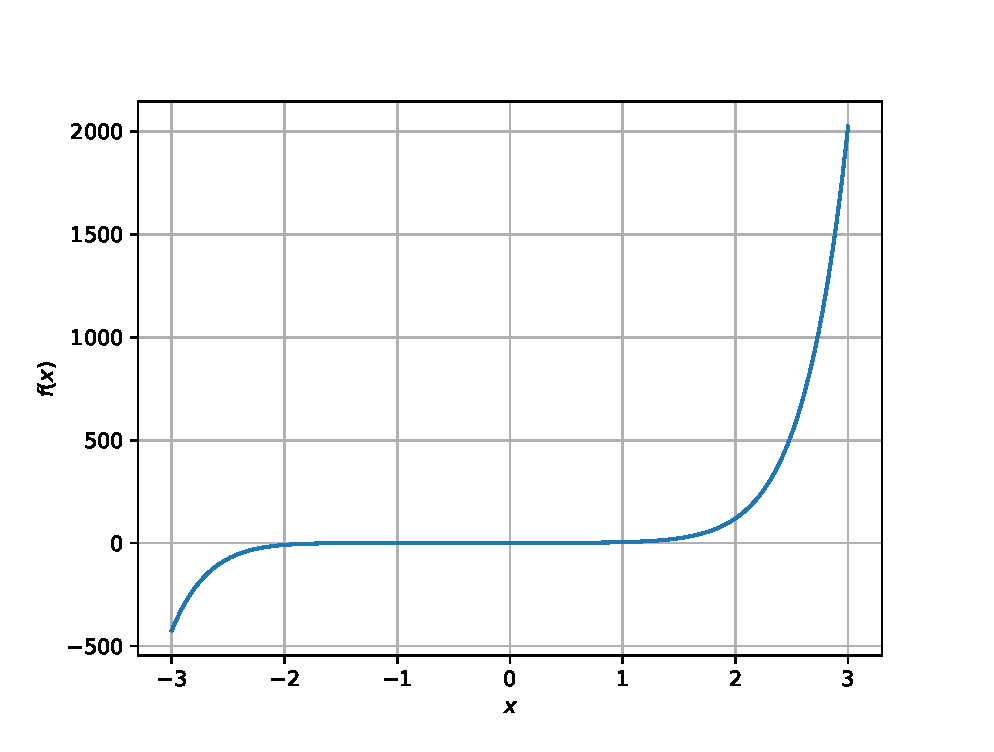
\includegraphics[width=\columnwidth]{./figs/1.eps}
\end{center}
\captionof{figure}{}

\label{fig:1}	
\end{figure}
\begin{definition}
\label{Uniform and point-wise convergence}
Let $D$ be a subset of $\mathbb{R}$ and let {$f_n$} be a sequence of real valued functions defined on $D$. Then {$f_n$} converges pointwise to $f$ if given any x in $D$ and given any $\epsilon>0$, there exists a natural number $N=N(x,\epsilon)$ such that $\abs{f_n(x)-f(x)}<\epsilon$ for every $n>N$.
The above definition implies uniform convergence if the inequality holds for every $x\in D$.
\end{definition}
\begin{problem}

For each $n \in \mathbb{N}$, let $f_n(x)=\brak{x-\frac{1}{n}}^2$ for $x\in[0,1]$. Find the following:
\begin{itemize}
\item Does $f_n$ converge pointwise on [0,1].
\item Does it converge uniformly.   	
\end{itemize}  
\solution
\begin{align}
\lim_{n \to \infty}f_n(x) = f(x) = x^2
\end{align} for $x$ in [0,1].
Consider $\abs{f_n(x)-f(x)}$. Since $x\in[0,1]$, there exists $n \in \mathbb{N}$ such that $x=\frac{1}{n}$
$\implies$ 
\begin{equation}
\abs{f_n(x)-f(x)} = \abs{f_n\brak{\frac{1}{n}}-f\brak{\frac{1}{n}}}   
\end{equation}
$\implies$
\begin{equation}
\abs{f_n(x)-f(x)}=\frac{1}{n^2}
\end{equation}
CLearly, $\frac{1}{n^2}$ is greater than $\epsilon$ for some values of $n$. So, $f_n(x)$ does not converge uniformly.
The following code proves our first result Fig. \ref{fig:1}.
\lstinputlisting{./codes/2.py}

\begin{figure}[!ht]
\begin{center}
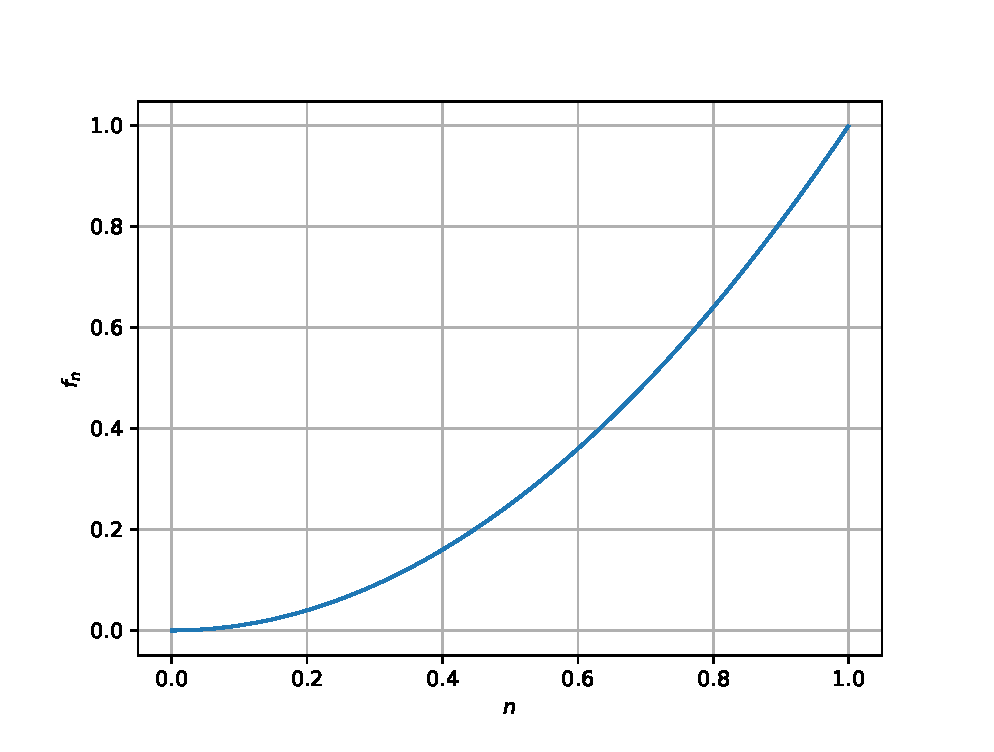
\includegraphics[width=\columnwidth]{./figs/2.eps}
\end{center}
\caption{}{}
\label{fig:1}	
\end{figure}
\end{problem}

%
\begin{definition}
\label{Taylor Series}
Taylor Series:
The taylor series of a $n$-time differentiable function $f(x)$ at a point $a$ is given by the following equation:
Note: Maclaurian series is nothing but taylor series of $f(x)$ at $x=0$.
\begin{equation}
f(x)=\sum_{n=0}^{\infty} \frac{f^n(a)}{n!}x^n
\end{equation}
\end{definition}
\begin{problem}
Obtain the taylor series of $f(x) = e^x$ at $x=0$.
\end{problem}
%%
\solution
Clearly, $f^n(0)=1$ for $f(x)=e^x$. So
\begin{equation}
f(x)=\sum_{n=0}^{\infty}\frac{1}{n!}x^n
\end{equation}
The following code plots  Fig. \ref{fig:2} verifying that the taylor expansion is indeed correct.
\lstinputlisting{./codes/3.py}
%
\begin{figure}[!ht]
\begin{center}
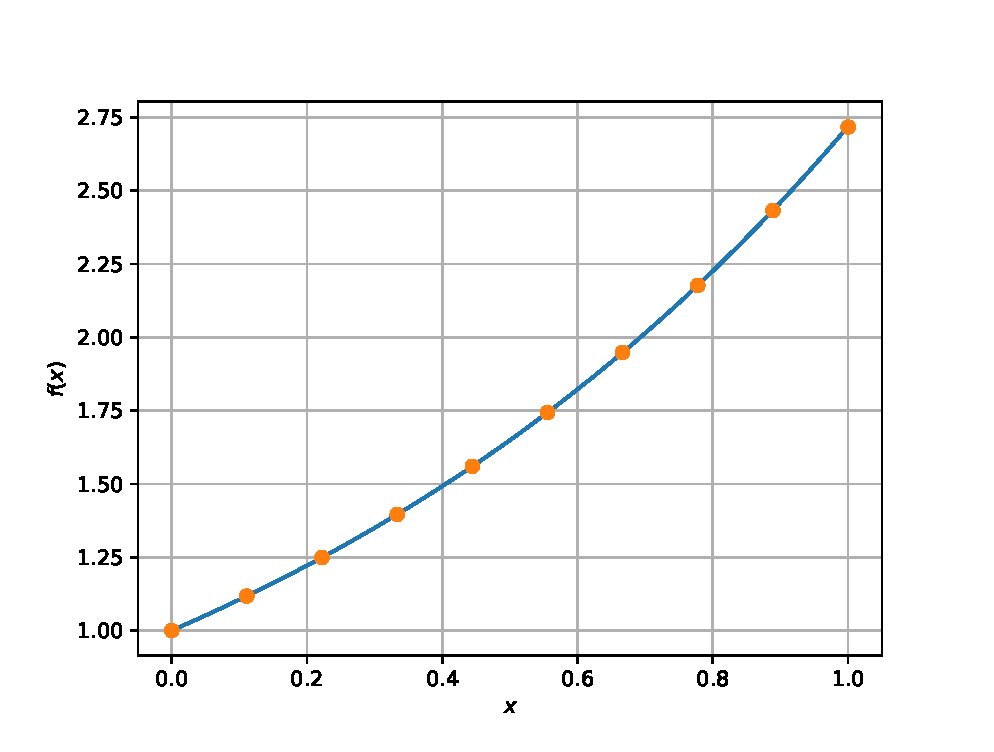
\includegraphics[width=\columnwidth]{./figs/3.eps}
\end{center}
\captionof{figure}{}
\label{fig:2}	
\end{figure}



\begin{definition}
\label{Fourier Series}
For a periodic function $f(x)$(with period $2L$), the fourier series is given by the following equation:
\begin{equation}
f(x)=a_0+\sum_{n=1}^{\infty}\brak{a_n\cos\brak{\frac{n\pi}{L}x}+b_n\sin\brak{\frac{n\pi}{L}x}}
\end{equation}
where the coefficients are given by:
\begin{equation}
a_0=\frac{1}{2L}\int_{-L}^{L}f(x)dx
\end{equation}
\begin{equation}
a_n=\frac{1}{L}\int_{-L}^{L}f(x)\cos\brak{nx}dx
\end{equation}
\begin{equation}
b_n=\frac{1}{L}\int_{-L}^{L}f(x)\sin\brak{nx}dx 
\end{equation}
where $n\ge1$. 
\end{definition}

\begin{problem}
Find the fourier series expansion of $f(x)=\sqrt{1-\cos x}$ on $(0,2\pi)$ and prove the following result:
\begin{equation}
\frac{1}{2}=\sum_{n=1}^{\infty}\frac{1}{4n^2-1}
\end{equation} 
\end{problem}
\solution 
Rewriting $f(x)$ interms of $\sin\brak{\frac{x}{2}} \implies f(x)=\sqrt{2}\sin\brak{\frac{x}{2}}$. Clearly, $\frac{x}{2} \in (0,\pi)$ where $\sin\brak{\frac{x}{2}}$ is positive. So, we need to expand $f(x)=\sqrt{2}\sin\brak{\frac{x}{2}}$. By careful application of \ref{Fourier Series}, we can conclude the following:
\begin{equation}
a_0=\frac{4\sqrt{2}}{\pi}
\end{equation}
\begin{equation}
a_n=\frac{-4\sqrt{2}}{\pi\brak{4n^2-1}}
\end{equation}  
and that $b_n=0$
$\implies$ \begin{equation}
\sqrt{1-cos x}=\frac{4\sqrt{2}}{\pi}-\sum_{n=1}^{\infty}\frac{4\sqrt{2}}{\pi\brak{4n^2-1}}
\end{equation}
$at x=0$, the equation becomes 
\begin{equation}
\frac{4\sqrt{2}}{\pi}=\sum_{n=1}^{\infty}\frac{4\sqrt{2}}{\pi\brak{4n^2-1}}
\end{equation}
\begin{equation}
\implies \frac{1}{2}=\sum_{n=1}^{\infty}\frac{1}{4n^2-1}
\end{equation}
Hence, proved. Some similar results can also be proved using fourier series.
\begin{problem}
Suppose 
\begin{equation}
f_n(x)=A_0+\sum_{k=1}^{n}\brak{A_k\cos kx + B_k\sin kx}
\end{equation}
be a trigonometric polynomial and $f(x)$ be a periodic function with period=$2\pi$. Show that if $f_n(x)$ minimises the integral $E=\int_{-\pi}^{\pi}\brak{f(x)-f_n(x)}^2$, then the coeffecients in $f_n(x)$ are same as the coefficients of the fourier series of $f(x)$.
\end{problem}
\begin{proof}
Let $a_0,a_1,...,a_n$ and $b_1,b_2,...,b_n$ be the fourier series coeffecients of $f(x)$. Consider the given integral. Expanding it gives $\int_{-\pi}^{\pi}\brak{f^2-2ff_n+{f_n}^2 dx}$. It can be trivially shown that the following equations hold true:
\begin{equation}
\int_{-\pi}^{\pi}\cos kx=0
\end{equation}
\begin{equation}
\int_{-\pi}^{\pi}\cos^2 kx=\pi
\end{equation}
\begin{equation}
\int_{-\pi}^{\pi}\cos kx\sin kx=0
\end{equation}
Same results hold true for $\sin kx$. We can prove the required result by using the above equations. Consider $\int_{-\pi}^{\pi}{f_n}^2 dx$. On applying the above equations and simplifying, we end up with the following expression:
\begin{equation}
\int_{-\pi}^{\pi}{f_n}^2 dx = \pi\brak{2A_0^2+\sum_{k=1}^{n}\brak{A_k^2+B_k^2}}
\end{equation}
On similar lines, we can get the following expression for $\int_{-\pi}^{\pi}ff_n dx$
\begin{equation}
\int_{-\pi}^{\pi}ff_n dx = 2\pi\brak{2A_0a_0+\sum_{k=1}^{n}\brak{A_ka_k+B_kb_k}}
\end{equation}
On careful observation, one can conclude that the above equation is nothing but the dot product between the vectors $(A_0,A_0,A_1,A_2,....,B_1,B_2,....),(a_0,a_0,a_1,a_2,...,b_1,b_2,....)$ whose maximum will minimise the error($\because$ it has a negative sign in the expansion). This happens only if all the corresponding components are equal. $\implies$ for minimum error, $A_k=a_k, 0 \le k\le n$.  
\end{proof}
\begin{problem}
Expand $\frac{1}{1+x^2}$ in powers of $x$ and hence find a power series expansion for $\tan^{-1} x$.
\end{problem}
\solution
The following code plots $\frac{1}{1+x^2}$ and its power series expansion in $(-1,1)$ which verifies our answer. 
\lstinputlisting{./codes/6.py}
%
\begin{figure}[!ht]
\begin{center}
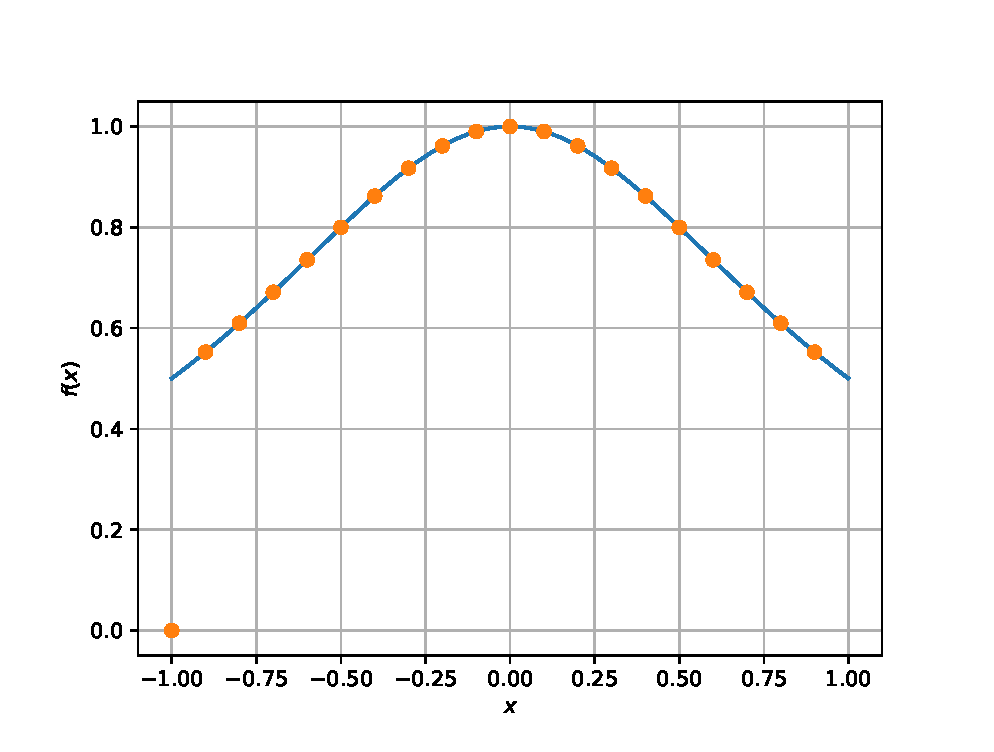
\includegraphics[width=\columnwidth]{./figs/6.eps}
\end{center}
%\caption{}{}
\label{fig:3}	
\end{figure}

$\because$ we are expanding in powers of $x$, we can safely assume that $\abs{x} < 1$. So, by using GP's infinite summation formula,
$\implies$ 
\begin{equation}
\frac{1}{1+x^2}=\frac{1}{1-(-x^2)}=1-x^2+x^4-x^6+.....(\infty)
\end{equation}
Integrating(indefinite) on both sides($\because$ both the sides of the equation are continuous),
$\implies$
\begin{equation}
\tan^{-1} x= x-\frac{x^3}{3}+\frac{x^5}{5}-\frac{x^7}{7}+....
\end{equation}
The above equation is the power series expansion for $\tan^{-1} x$ at $x=0$. The following figure verifies the above equation.
\lstinputlisting{./codes/7.py}
\begin{figure}[!ht]
\begin{center}
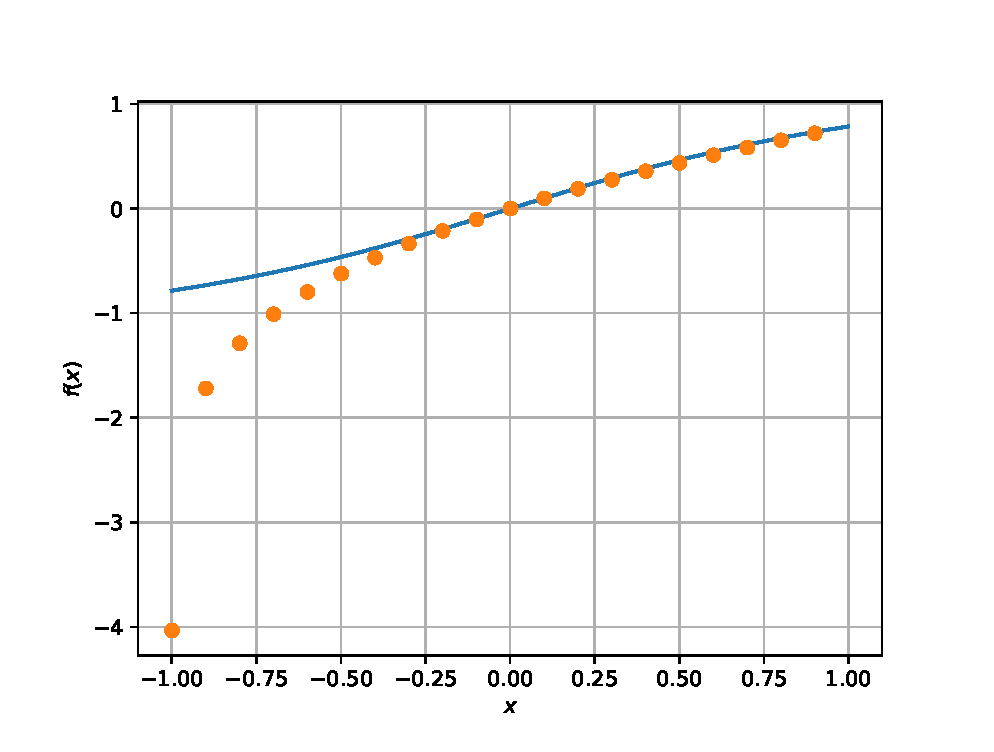
\includegraphics[width=\columnwidth]{./figs/7.eps}
\end{center}
%\caption{figure}{}
\label{fig:4}	
\end{figure}
\begin{definition}
Riemann Sum:
Suppose $f:[a,b] \to R$ and partition $P={[x_0,x_1],[x_1,x_2],....,[x_{n-1},x_n]}$, then the sum $S=\sum_{i=1}^{n}f(x^*_i)\Delta x_i$ is called Riemann Sum over the interval $[a,b]$ whose limit at $\infty$ gives the definite integral of $f(x)$ over the interval $[a,b]$. 
\end{definition}
\begin{problem}
Evaluate $\int_{a}^{b} e^{x} dx$ using Riemann Sum method.
\end{problem}
\solution
Let $x^*_i=a+i\Delta x$ where $\Delta x=\frac{b-a}{n}$ where $n$ is the number of partitions.
$\implies f(x^*_i)=e^{a}e^{i\Delta x}$. Doing the summation, from 0 to $n$ gives the following equation:
\begin{equation}
\sum_{i=1}^{n}f(x^*_i)\Delta x_i=e^a\brak{\frac{e^{b-a}-1}{\frac{e^{\frac{b-a}{n}}-1}{\frac{b-a}{n}}}}
\end{equation}
On applying the limit($n \to \infty$), the summation boils down to $e^b-e^a$ which is the required value($\because$ the denominator tends to 1 as $n \to \infty$).
\begin{definition}
\label{Improper Integrals and convergence}
In mathematical analysis, an improper integral is the limit of a definite integral as an endpoint of the interval(s) of integration approaches either a specified real number or $\infty$ or $-\infty$ or, in some cases, as both endpoints approach limits.
Symbolically, it is written as follows:
\begin{equation}
\lim_{b \to \infty}\int_{a}^{b}f(x) dx, \lim_{a \to -\infty}\int_{a}^{b}f(x) dx
\end{equation}
Similar representation can be given for integrals over finite intervals. If the limit value is finite, then the integral is said to converge to that finite value. 
\end{definition}
\begin{problem}
Comment on the convergence of $\int_{0}^{\infty}x \sin x$.
\end{problem}
\solution
Consider the following integral $\int_{0}^{t}x \sin x$
$\implies$\begin{equation}
\int_{0}^{t}x \sin x = -t\cos t + \sin t
\end{equation} 
Clearly as $t \to \infty$, the value of the integral diverges to $-\infty$. $\therefore$ the integral diverges.
\begin{proposition}
\label{Gamma function}
The function of the form $\int_{0}^{\infty}t^{s-1} e^{-t} dt, s>0$ is called the gamma function. It is denoted by $\Gamma(s)$.
\end{proposition}
\begin{problem}
Discuss the convergence of $\Gamma$ function and prove that $\Gamma(n+1)=n!$.
\end{problem}
\solution
Using \ref{Gamma function}, 
\begin{equation}
\Gamma(s)=\int_{0}^{\infty}t^{s-1} e^{-t} dt=\int_{0}^{1}t^{s-1} e^{-t} dt+\int_{1}^{\infty}t^{s-1} e^{-t} dt
\end{equation}
Here $\int_{0}^{1}t^{s-1} e^{-t} dt < \int_{0}^{1}t^{s-1} dt$ which converges to $\frac{1}{s}$.
For the second term, we can use the fact that exponential function grows faster than any polynomial. So, $\exists N$ such that for $t\ge N$, $t^{s-1}<e^{\frac{t}{2}}$. Again the integral can be split as 
\begin{equation}
\int_{1}^{\infty}t^{s-1} e^{-t} dt = \int_{1}^{N}t^{s-1} e^{-t} dt + \int_{N}^{\infty}t^{s-1} e^{-t} dt 
\end{equation}
which is less than 
\begin{equation}
\int_{1}^{N}t^{s-1} e^{-t} dt + \int_{N}^{\infty} e^{-t/2} dt
\end{equation}
Clearly, the above equation takes a finite value. So, $\int_{1}^{\infty}t^{s-1} e^{-t} dt<\infty$. $\therefore$ $\Gamma$ function converges.
On applying integration by parts and simplifying we end up with the following equation
\begin{equation}
\Gamma(n)=(n-1)\Gamma(n-1)=(n-1)!\Gamma(1)
\end{equation}
It is trivial that $\Gamma(1)=1$. So, $\Gamma(n)=(n-1)!$ which $\implies$ $\Gamma(n+1)=n!$. 
\begin{problem}
Calculate the following for the cycloid formed by $x=r(t-\sin t),y=r(1-\cos t)$
\begin{itemize}
\item Arc length of one arc($0 \le t \le 2\pi$)
\item Surface area of the solid generated by rotating this arc about the $x-$ axis. 
\end{itemize}
\end{problem}      
\solution
The following code plots the given curve for $0 \le t \le 2\pi$.
\lstinputlisting{./codes/8.py}
\begin{figure}[!ht]
\begin{center}
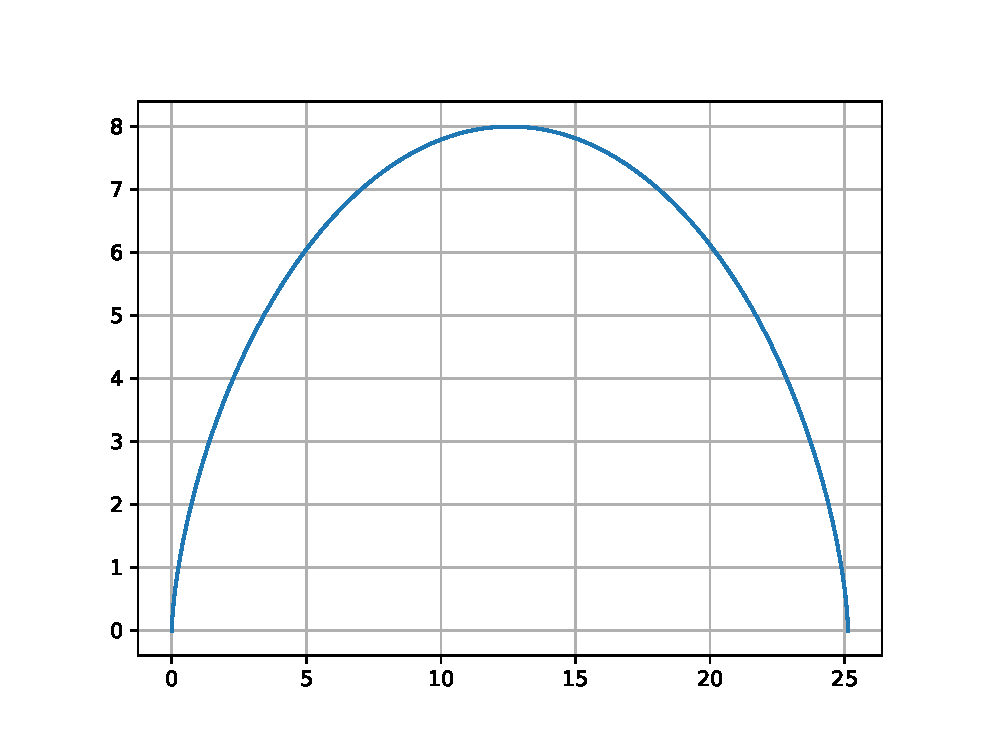
\includegraphics[width=\columnwidth]{./figs/8.eps}
\end{center}
%\caption{figure}{}
\label{fig:4}	
\end{figure}
We know that $dr=\sqrt{\brak{\frac{dx}{dt}}^2+\brak{\frac{dy}{dt}}^2} dt$. So, total arc length is nothing but $\int_{0}^{2\pi} dr$. By careful simplification, we get:
\begin{equation}
\frac{dx}{dt}=r(1-\cos t)	
\end{equation}
\begin{equation}
\frac{dy}{dt}=r\sin t
\end{equation}
Substituting the above in the required integral yields
\begin{equation}
\int_{0}^{2\pi}2r \sin \frac{t}{2}
\end{equation}
Whose value is $8r$. So, the arc length is $8r$.
The surface area is given by the integral $\int_{0}^{2\pi} 2\pi y dr$. So, the surface area=$\int_{0}^{2\pi} 2   \pi 2r^2(1-\cos t)\sin \frac{t}{2}$. On proper simplification, this integral yields $8 \pi r^2$.
So, the arc length is $8r$ and the surface area is $8 \pi r^2$. 
\begin{proposition}
\label{Lebesegue's Dominated convergence theorem}
Let $f_n(x)$ be a sequence of integrable functions on $I$ such that each $f_n$ is non-negative on $I$ and $f_n$ converges(pointwise) to $f$. Then $f_n$ is said to be dominantly convergent on $I$ if there is some other integrable function on $I$ such that $\abs{f(x)}<g(x)$ almost everywhere on $I$.
The above implies that 
\begin{equation}
\lim_{n \to \infty}\int_{I}f_n(x) dx=\int_{I}\lim_{n \to \infty}f_n(x) dx
\end{equation}
Similar kind of definition is applicable for series.
\end{proposition}
\begin{problem}
Prove or disprove that the series $\sum_{n=1}^{\infty}\frac{x^n}{n}$ is dominant on $[0,1]$.
\end{problem}
\solution
By \ref{def: Interval and Radius of convergence}, it is clear that the given series converges in $[0,1]$. Also,
\begin{equation}
\sum_{n=1}^{\infty}\frac{x^n}{n} < \sum_{n=1}^{\infty} x^n
\end{equation}
$\because x<1$,  
\begin{equation}
\sum_{n=1}^{\infty} x^n = \frac{x}{1-x}
\end{equation}
The above function is integrable on $[0,1]$ and we also know that the series converges to some function $f$ which will be less than $\frac{x}{1-x}$.
$\therefore$ the above function is dominated on $[0,1]$.
\end{document}

